\documentclass[conference]{IEEEtran}
\usepackage[T1]{fontenc}
\usepackage{amsmath,amssymb}
\usepackage{graphicx}
\usepackage{booktabs}
\usepackage{multirow}
\usepackage{xcolor}
\usepackage[hidelinks]{hyperref}
\usepackage{url}
\usepackage{cite}
\usepackage{balance}

\newcommand{\K}{\mathbf{K}}
\graphicspath{{figs/}}

\begin{document}

\title{Steering the Linux Scheduler with\\ Koopman Burst Prediction under EEVDF}

\author{\IEEEauthorblockN{Saarthak Manocha}
\IEEEauthorblockA{Dept. of Information Technology\\
Chaitanya Bharathi Institute of Technology\\
Hyderabad, India\\
saarthakmanocha@gmail.com}}

\maketitle

\begin{abstract}
Shortest-job-first scheduling needs each task's next CPU burst before it runs. We predict bursts with a Koopman operator, fitted by dynamic mode decomposition on log-scale delay coordinates, and feed the predictions to the unmodified Linux EEVDF scheduler as per-task slice requests. Every measurement is validated against the kernel's own accounting (CPU time within 0.93\%, wait within 0.22\%, 105 processes). On real programs (Redis, SQLite, Node.js, ffmpeg) the predictor beats the textbook exponential average in 32 of 36 threads, with 29\% lower error. We show it is numerically a log-scale autoregressive model, and that neither nonlinear observables, ARIMA nor a neural network beat that model. Closing the loop with an eBPF observer that costs 0.33\% of one core, predicted slices cut short-request response time by 45\% with no loss of throughput, and the Koopman predictor beats the exponential average in 19 of 24 paired runs. We show why slices need a margin above the predicted burst: an exact slice gives no gain, 1.5 times the burst gives 61\%. With real servers sharing a core with CPU hogs, Redis requests became 31--37\% faster and SQLite point queries 31\% faster, with tail latency unchanged. We release the capture kit, data, controller, a sched\_ext policy for bare-metal tests and a scheduler visualizer.
\end{abstract}

\begin{IEEEkeywords}
Koopman operator, dynamic mode decomposition, CPU scheduling, EEVDF, shortest job first, eBPF, kernel tracing, conformal prediction
\end{IEEEkeywords}

\section{Introduction}
Shortest-job-first (SJF) scheduling minimizes mean waiting time, but it needs the length of each task's next CPU burst before the burst runs. Textbooks teach an estimate, the exponential average $\tau_{n+1}=\alpha t_n+(1-\alpha)\tau_n$~\cite{silberschatz2018}, and production schedulers avoid prediction: Linux's fair class has, since kernel~6.6, picked the task with the earliest eligible virtual deadline (EEVDF)~\cite{stoica1995,corbet2023eevdf}. Since kernel 6.12, however, EEVDF lets each task request its own time slice, and a shorter slice means an earlier deadline~\cite{corbet2024,eevdfdoc}. That turns burst prediction from a textbook exercise into a lever on a production scheduler: if a task's next burst is known, its slice can be set to match.

We ask three questions with real kernel data. Can bursts be predicted better than with the textbook estimator? Does a better prediction make the real scheduler faster? And what, specifically, does a Koopman view add? Koopman operator theory~\cite{koopman1931,mezic2005,brunton2022} represents a nonlinear system by a linear operator on functions of its state; dynamic mode decomposition (DMD) and its extension EDMD~\cite{schmid2010,williams2015} estimate it from data, and its eigenvalues describe how patterns decay. Applied to delay coordinates (Hankel DMD) it is closely related to autoregressive models~\cite{arbabi2017,pan2020}; we test whether, for CPU bursts, it is more than that.

\textbf{Contributions.}
\begin{enumerate}
\item A validated measurement pipeline for scheduler dynamics: capture without perturbation, ground truth from \texttt{schedstat}, and two documented measurement hazards (Section~\ref{sec:measure}).
\item Burst prediction on synthetic workloads and four real programs against autoregressive, ARIMA, neural and nonlinear-Koopman baselines, with prediction intervals and cost (Section~\ref{sec:pred}).
\item A closed-loop controller that steers unmodified EEVDF through slice requests, first by polling and then with an eBPF observer, evaluated in 264 paired runs including real servers, with a model of why slices need a margin (Sections~\ref{sec:method} and~\ref{sec:closed}).
\item Multi-core analysis, a machine-level change detector, a trace visualizer, and a sched\_ext policy for bare-metal tests (Sections~\ref{sec:multicore}--\ref{sec:viz}).
\end{enumerate}

\section{Background and Related Work}
\textbf{Koopman operators and DMD.} For a map $x_{t+1}=F(x_t)$ the Koopman operator advances observables, $(\mathcal{K}g)(x)=g(F(x))$, linearly even when $F$ is not~\cite{koopman1931}. EDMD approximates it by the matrix $\K$ minimizing $\|\Psi_Y-\Psi_X\K\|_F$ over snapshot pairs of a dictionary $\psi$~\cite{williams2015}; with $\psi(x)=x$ it is DMD~\cite{schmid2010,tu2014}, and it converges to the projection of $\mathcal{K}$ onto the dictionary span~\cite{korda2018}. Delay coordinates are justified by Takens' theorem~\cite{takens1981,arbabi2017}; linear models on them include AR models and Hankel DMD as special cases~\cite{pan2020}. Noise biases eigenvalues towards zero~\cite{dawson2016}.

\textbf{Learning in schedulers.} Negi and Kumar predicted CPU bursts from process attributes with decision trees and set Linux~2.4 time slices from them, reducing turnaround by 1.4--5.8\%~\cite{negi2005}. Size-based scheduling helps heavy-tailed workloads~\cite{harchol2003}. sched\_ext (6.12) lets BPF programs implement scheduling policies~\cite{schedext}; recent work uses a learned classifier to switch between whole sched\_ext policies~\cite{wang2025mos}. EEVDF slice requests were added so that latency-sensitive tasks can be served sooner, at some cost to throughput if slices are too short~\cite{corbet2024}. We know of no study that sets them from predicted bursts.

\section{Method}\label{sec:method}
\textbf{Predictor.} For each task, the state is its last three bursts on a log scale, $z_t=(\log b_t,\log b_{t-1},\log b_{t-2})$, standardized with training statistics, and one operator is fitted by least squares, $\K=\arg\min_A\sum_t\|z_{t+1}-z_tA\|^2$. The predicted burst is the first coordinate of $z_t\K$, mapped back. Because the dictionary is linear in delay coordinates, this is numerically a log-scale AR(3) model: the two give the same forecasts (median of the largest log-space difference $10^{-3}$ over 96 tasks). We call it log-EDMD and also test nonlinear dictionaries: squares and products of the lags (\emph{poly}) and 64 random Fourier features (\emph{RFF}, approximate kernel EDMD). In the controller the operator is updated after every burst by recursive least squares with forgetting factor 0.995. The eigenvalues of $\K$ describe each task's burst dynamics.

\textbf{From prediction to slice.} The slice requested for a task is $s=c\,\hat b$, clamped between the kernel minimum (0.1\,ms) and the default slice (1.4\,ms here), where $\hat b$ is the predicted burst and $c$ a margin. All tasks have equal weight.

\textbf{Why a margin.} Under EEVDF a woken task gets virtual deadline $v+s$. A smaller $s$ makes it more likely to preempt the running task at once (allowed when its slice is shorter and its deadline earlier) and to be picked next, so its wait $W(s)$ grows with $s$. But if its actual CPU demand $b'$ (the burst plus system overhead) exceeds $s$, its deadline is renewed while it still runs and it loses its place to tasks with earlier deadlines, an extra wait $\Delta$ of the order of their slices. So
\begin{equation}
\mathbb{E}[R\mid s]\approx W(s)+b'+\Delta\,\Pr(b'>s),
\end{equation}
and with $s=c\hat b$ and log-normal prediction error of spread $\sigma$, $\Pr(b'>s)\approx1-\Phi(\log c/\sigma)$ when the overhead is small. Two consequences follow. Even a perfect predictor needs $c>1$, because $b'>b$. And at a given margin, a predictor with smaller $\sigma$ overruns less, so differences between predictors should show at small $c$ and vanish at large $c$, where slices saturate at the default. Section~\ref{sec:closed} tests both.

\section{Measurement and Validation}\label{sec:measure}
\begin{table}[t]
\centering
\caption{Platforms and data}\label{tab:platforms}
\setlength{\tabcolsep}{3pt}
\begin{tabular}{@{}llll@{}}
\toprule
Platform & Kernel & Capture & Runs \\
\midrule
Lab, 28 CPUs, bare metal & 7.0 & perf & 1 (75\,s) \\
Intel Xeon VM, 2 vCPUs (KVM) & 6.18 & tracefs & 12 + 24 + 3 \\
\quad same VM, closed loop & 6.18 & counters, eBPF & 264 \\
ARM VM, 4 vCPUs (Apple host) & 6.8 & counters & 9 + 24 \\
\bottomrule
\end{tabular}
\end{table}

\textbf{Platforms and workloads} (Table~\ref{tab:platforms}). All kernels run EEVDF. Synthetic workloads are a CPU-bound loop, an I/O-bound loop that writes 10\,kB and sleeps 50\,ms, and a \emph{phased} positive control alternating every 2\,s between 1\,ms and 20\,ms bursts. The lab trace (\emph{Trace~3}) ran three CPU-bound and three I/O-bound jobs; VM captures ran these plus two phased jobs, pinned to 1 or 2 cores, overloaded, or with a load drop, three times each. Real programs and the closed-loop workloads are described in Sections~\ref{sec:pred} and~\ref{sec:closed}.

\textbf{Reconstruction and ground truth.} From \texttt{sched\_switch}, \texttt{sched\_wakeup} and \texttt{sched\_migrate\_task} events we rebuild, per task, every interval on a CPU (with its state at switch-out), every interval waiting in a run queue, and every migration. A burst is the CPU time between two blocking events. Each workload saves the kernel's own \texttt{/proc/self/schedstat} and context-switch counts before it exits. Over 105 processes in 12 VM captures (Fig.~\ref{fig:valid}), reconstructed CPU time differs from the kernel's by 0.93\% (median; max 3.45\%), wait time by 0.22\% (max 2.07\%), and the number of times scheduled by a median of 4, with no lost events.

\begin{figure}[t]
\centering
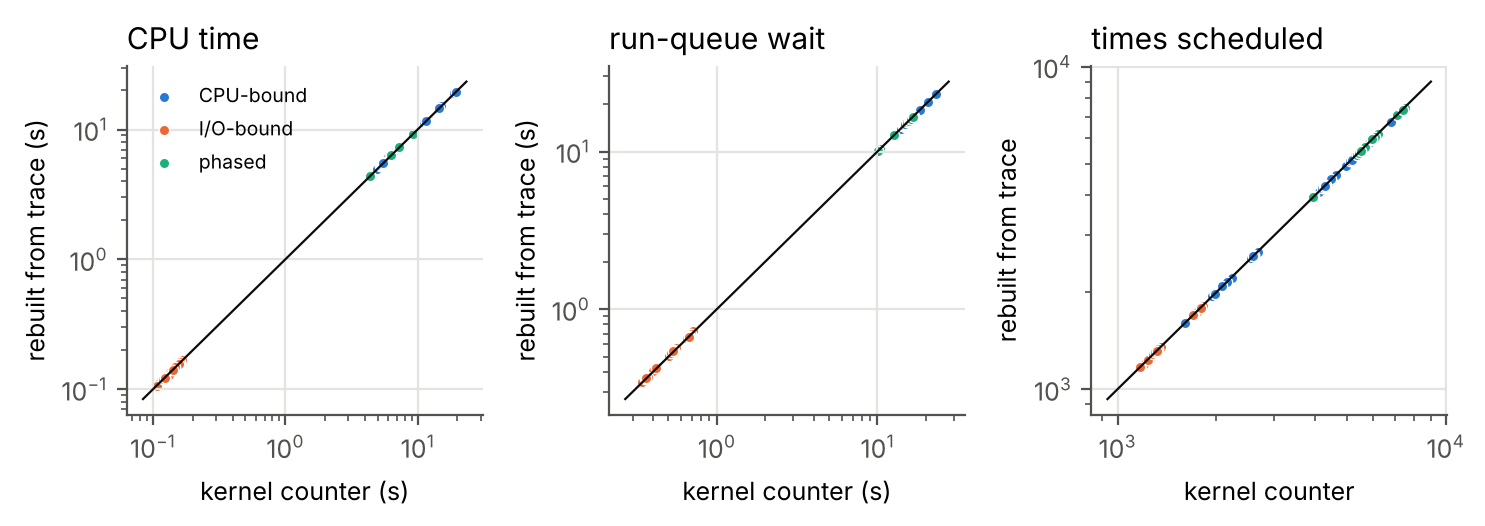
\includegraphics[width=\columnwidth]{m1_validation.png}
\caption{Every reconstructed process against the kernel's own counters (105 processes, 12 captures).}\label{fig:valid}
\end{figure}

\textbf{Hazard 1: the observer effect.} A first capture tool streamed events while recording. Each event woke the reader, which preempted the workload and produced further events: about 50{,}000 context switches per second on any core with spare capacity, traces 20--30 times larger, and counts off by up to 9\%. Recording into a large kernel buffer and reading it after the run removed it.

\textbf{Hazard 2: missing idle exits on a VM.} On the Intel VM's kernel, part of the \texttt{sched\_switch} events for a CPU leaving idle are never emitted (tracefs and perf agree; the ring buffer reports no loss): a task that slept 201 times was seen switching in only 1 to 176 times across seven self-tests. The lab machine does not show it. Our tools count unmatched switch-outs and keep VM cores busy, with workload or with one lowest-priority (\texttt{SCHED\_IDLE}) spinner per core, after which counts match the kernel.

\section{Burst Prediction}\label{sec:pred}
\textbf{Protocol.} Every method predicts a burst from earlier bursts of the same task; the last 20\% of each task is the test set. Methods: mean, last value, the textbook exponential average ($\alpha=0.5$, EWMA) and with tuned $\alpha$, log-EDMD, poly- and RFF-EDMD, log-AR with order 1--10 chosen by AIC (log-AR($p^*$)), ARIMA chosen by AIC, a two-layer neural network on six log lags, and gradient boosting on three raw lags. Intervals are moving-block bootstrap~\cite{kunsch1989}; sign tests are Holm-corrected~\cite{holm1979}.

\textbf{Synthetic workloads.} On the idle 28-core lab machine, I/O bursts tripled on the same cores when the CPU-bound jobs exited (Fig.~\ref{fig:trace3}), a level shift that the exponential average follows best; the I/O operators' dominant eigenvalues, 0.88--0.97, mark it. Under contention on the VM, the positive control's structured bursts are captured by every method that uses recent bursts (90--96\% lower error than the mean), best by tuned EWMA; log-EDMD is 5--23\% worse there. On contended I/O bursts the order reverses: log-EDMD beats EWMA in 33 of 33 processes (median error ratio 0.86, $p_\text{Holm}=2\times10^{-9}$), because the exponential average overreacts to single long bursts.

\begin{figure}[t]
\centering
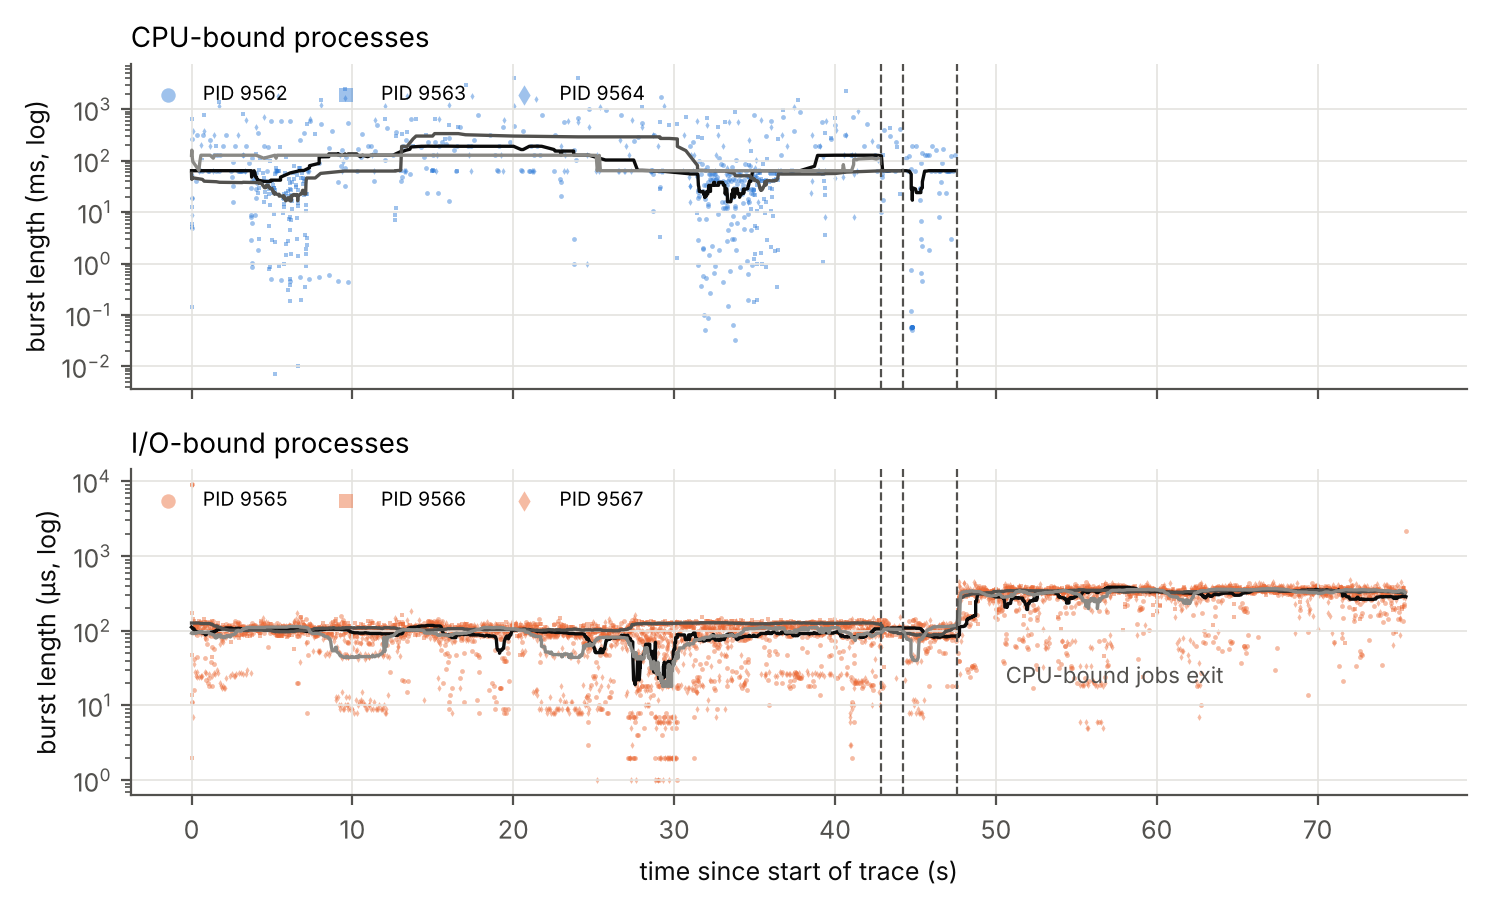
\includegraphics[width=\columnwidth]{fig2_burst_timeline.png}
\caption{Trace~3 (bare metal, 28 cores): every burst over time. I/O bursts lengthen about threefold when the CPU-bound jobs exit (dashed lines).}\label{fig:trace3}
\end{figure}

\textbf{Real programs.} We traced, together on both VM cores for three 60\,s captures, a Redis~7.0 server driven by a paced client, a Node.js~22 HTTP server with phases of light and heavy JSON requests, SQL queries of mixed size against SQLite~3.45, real-time H.264 encoding with ffmpeg (all threads), and the load generators, with a gcc build and xz compression as background load. Over the 36 threads with at least 60 bursts, CPU time agrees with \texttt{schedstat} within 1.8\% and wait within 1.5\% (medians). Log-EDMD beats EWMA in 32 of 36 threads, with median error ratio 0.71 ($p_\text{Holm}=10^{-5}$; Fig.~\ref{fig:real}); the gain is largest for Redis and SQLite (0.55 and 0.56), whose short request bursts are interrupted by occasional long ones.

\begin{figure}[t]
\centering
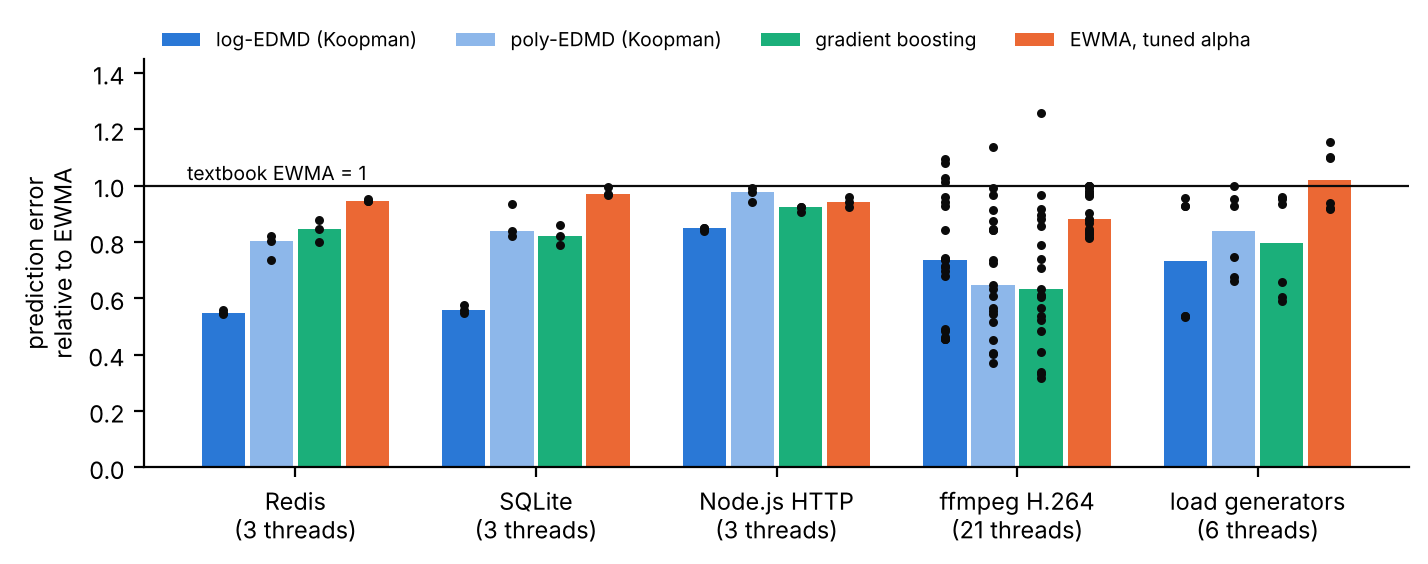
\includegraphics[width=\columnwidth]{e8_real_programs.png}
\caption{Real programs: burst-prediction error relative to the textbook exponential average (bars: median; dots: threads; three captures).}\label{fig:real}
\end{figure}

\begin{table}[t]
\centering
\caption{Is it more than an AR model? Median error ratio and number of tasks where the method is better, against two references (96 tasks, 36 of them threads of real programs)}\label{tab:baselines}
\setlength{\tabcolsep}{3pt}
\begin{tabular}{@{}lcccc@{}}
\toprule
 & \multicolumn{2}{c}{vs EWMA} & \multicolumn{2}{c}{vs log-AR($p^*$)} \\
Method & all 96 & real 36 & all 96 & real 36 \\
\midrule
log-EDMD (3 delays) & 0.88, 65 & 0.71, 32 & 1.02, 21 & 1.01, 8 \\
log-AR($p^*$), AIC & 0.79, 66 & 0.70, 32 & -- & -- \\
poly-EDMD & 0.86, 68 & 0.71, 35 & 1.01, 41 & 1.00, 20 \\
RFF-EDMD (kernel) & 0.85, 60 & 0.74, 28 & 1.00, 46 & 1.00, 20 \\
ARIMA, AIC & 0.85, 66 & 0.71, 33 & 1.02, 31 & 1.00, 15 \\
neural network & 0.84, 66 & 0.74, 32 & 1.02, 34 & 1.00, 18 \\
gradient boosting & 0.87, 68 & 0.79, 34 & 1.03, 33 & 1.04, 14 \\
\bottomrule
\end{tabular}
\end{table}

\textbf{Is it more than an AR model?} Table~\ref{tab:baselines} answers no. Every model that uses recent bursts beats the textbook estimator, all by similar amounts. The best single family is a log-scale linear model with enough delays: log-AR with AIC-chosen order (most often 10) is better than log-EDMD with three delays in 75 of 96 tasks, though only by 1.5\% at the median; this is Hankel DMD with more delay coordinates. Nonlinear dictionaries, ARIMA, the neural network and gradient boosting do not beat it (Holm $p\geq0.37$ for the two nonlinear Koopman variants). What predicts CPU bursts is the log scale and the delay depth, not nonlinearity. The Koopman view contributes the eigenvalues: fitted on windows of 150 bursts, they alone identify which of the five programs a window came from with 76\% balanced accuracy (chance 20\%; SQLite's are all real, the load generators' slowest mode is 0.87), though simple burst statistics do better (99.8\%).

\textbf{Uncertainty and cost.} Split conformal prediction~\cite{vovk2005,angelopoulos2023} on log-errors gave the target 90\% coverage (median 0.90 for log-EDMD, 0.91 for EWMA on I/O tasks), with narrower intervals for log-EDMD in 34 of 60 tasks (median width ratio 0.84). In C, one prediction takes 5.6\,ns and a recursive-least-squares update 29\,ns, less than a context switch.

\section{Closing the Loop: Steering EEVDF}\label{sec:closed}
\textbf{Workload.} Request tasks (C) wake on a period of 15--25\,ms and do one CPU burst each, drawn from a two-regime log-autoregressive process (short bursts near 0.3\,ms, long ones near 4\,ms, switching with probability 0.05), logging deadline, wake-up and finish; CPU hogs spin and count the CPU time they get. Every repetition runs every policy with the same seeds in shuffled order. The tasks' own CPU accounting agrees with \texttt{schedstat} within about 1\% (median). The main metric is the mean response time of short requests (under 1\,ms of CPU), from deadline to finish.

\textbf{Polling agent.} A first agent polled \texttt{/proc} every 10\,ms. On one CPU (three hogs, four request tasks, eight repetitions) and two CPUs (six and eight, six repetitions; 635{,}531 requests in all), both predictors cut short-request response in every paired repetition, by 28--31\% (Wilcoxon $p=0.008$ and $0.03$, the smallest attainable), at a 3--7\% throughput cost that equals the agent's own CPU time. Hand-set 0.1\,ms slices for the request tasks cut wake-up latency but not response ($-3\%$): every burst is chopped into 0.1\,ms pieces, with 7--8 times more context switches.

\begin{figure*}[t]
\centering
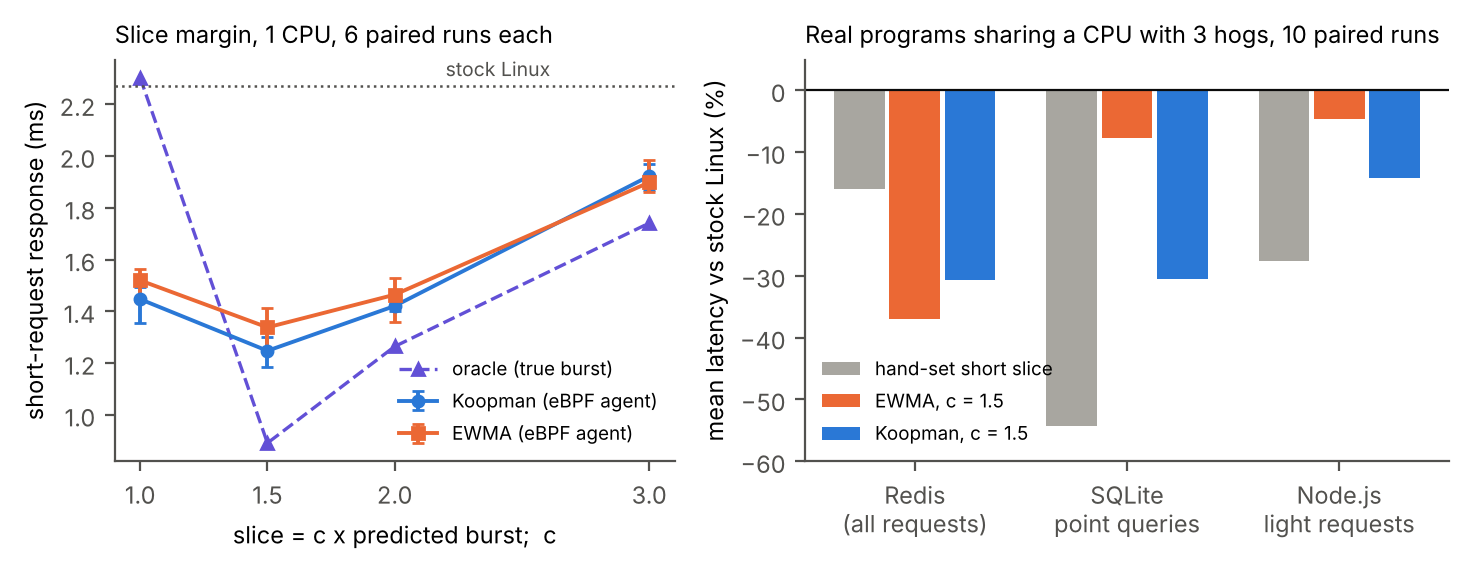
\includegraphics[width=0.86\textwidth]{e9_margin_real.png}
\caption{Left: short-request response against the slice margin $c$ (eBPF agent, one CPU with three hogs; bars: range over six paired runs); the oracle knows each burst exactly. Right: change in mean latency of real programs sharing one CPU with three hogs (ten paired runs), against stock EEVDF.}\label{fig:closed}
\end{figure*}

\textbf{eBPF agent.} A BPF program on the \texttt{sched\_switch} tracepoint reports every burst the moment it ends, and a C agent updates the task's predictor and sets its slice. It uses 0.33\% of one core, against 3\% for the polling agent, and CPU hogs lose no measurable throughput (within $\pm1\%$ of stock). Fig.~\ref{fig:closed} (left) sweeps the margin, and both predictions of the model hold. The oracle with $c=1$ is no better than stock Linux (+1.5\%), while $c=1.5$ gives $-61\%$ and larger margins lose ground ($-44\%$ at 2, $-23\%$ at 3). The predictors follow the same curve, with the best margin also at 1.5: Koopman $-45\%$ (1.25 against 2.27\,ms), EWMA $-41\%$, and mean response over \emph{all} requests $-5$ to $-6\%$. Koopman beats EWMA in 6 of 6 paired runs at $c=1$ and at $c=1.5$ ($p=0.031$ each), 5 of 6 at 2, and 2 of 6 at 3; over all margins in 19 of 24 ($p=0.0035$). Its burst predictions are 9\% more accurate (mean absolute error 0.77 against 0.84\,ms; log-error spread 0.49 against 0.58).

\textbf{Real programs.} A Redis server, a Node.js server and a SQLite worker shared one CPU with three hogs, with their clients on the other CPU timing every request end to end; the agent controlled the three server threads (ten paired repetitions; Fig.~\ref{fig:closed}, right). With predicted slices at $c=1.5$, Redis request latency fell by 31\% (Koopman) and 37\% (EWMA), SQLite point queries by 31\% and 8\%, and Node.js light requests by 14\% ($p=0.01$) and 5\% (not significant); the Koopman changes for Redis and SQLite held in 10 of 10 pairs ($p=0.002$). Koopman was 25\% better than EWMA on SQLite point queries (10 of 10) and 10\% worse on Redis (1 of 10). With either predictor at $c=1.5$, the mean over all Node.js and SQLite requests, heavy requests, and the 99th percentiles of all three programs changed by less than 4\% (not significant), and hogs lost 1\% of CPU time. Hand-set minimum slices for the servers did best for SQLite point queries ($-54\%$) and Node.js light requests ($-28\%$) but worst for Redis ($-16\%$), and require knowing which tasks are latency-sensitive.

\section{Multi-Core Scheduling}\label{sec:multicore}
On the lab machine, processes waited a median 16\,$\mu$s for a CPU: no queue formed, so no pick order could matter. On the ARM VM, from kernel counters alone, CPU-bound jobs spent 76\% of their time waiting on one core, 50\% on two and 1\% on four; the Intel VM traces agree. A trace-driven simulator replaying each traced task's real bursts and blocking times under FCFS, round robin, non-preemptive SJF and SRTF with each predictor (Fig.~\ref{fig:cores}) shows I/O response time zero for every policy once cores outnumber CPU-bound jobs. Below that, non-preemptive SJF behaves like FCFS whatever the predictor (10.2 against 10.4\,ms at two cores), because an I/O job must wait for the CPU-bound job holding the core; SRTF with any predictor brings it to 0.011\,ms. Measured EEVDF on one core gave interactive jobs 1.87\,ms against 1.5--1.9\,ms for simulated SRTF with predictors. Prediction pays only where tasks queue, and only through preemption, which is what slice requests provide.

\begin{figure}[t]
\centering
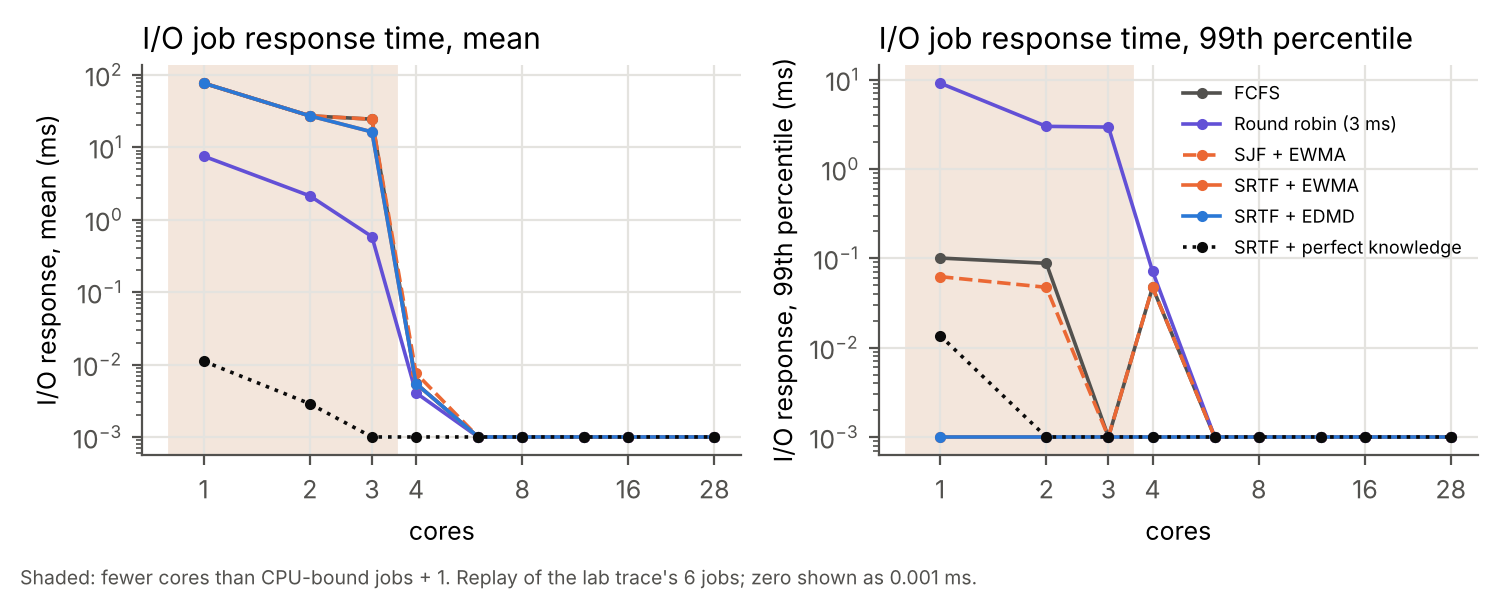
\includegraphics[width=\columnwidth]{m2_cores_vs_policy.png}
\caption{Simulated I/O response time versus core count, replaying the lab trace's six jobs.}\label{fig:cores}
\end{figure}

\section{Koopman View of the Whole Machine}\label{sec:detect}
The same estimator applied to a machine-wide state (busy fraction and queued tasks per core, CPU share per job class, every 10\,ms) detects load changes from its one-step residual. In three VM runs where four of six CPU-bound jobs stop while every core stays busy, it raised an alarm 77--94\,ms after the change, with no false alarm before it or in nine runs without a change; utilization, persistence and distance-from-normal monitors detected none (Fig.~\ref{fig:regime}). A live version reading only \texttt{/proc/stat}, unprivileged and at 0.5--1.1\% of one core, detected 29 of 36 scripted changes on two VMs with a median delay of 0.18\,s, but a static distance-from-normal score on the same three variables was as good or better in 51 of 54 settings: on low-dimensional counters, watching the variables jointly matters more than modelling their dynamics.

\begin{figure}[t]
\centering
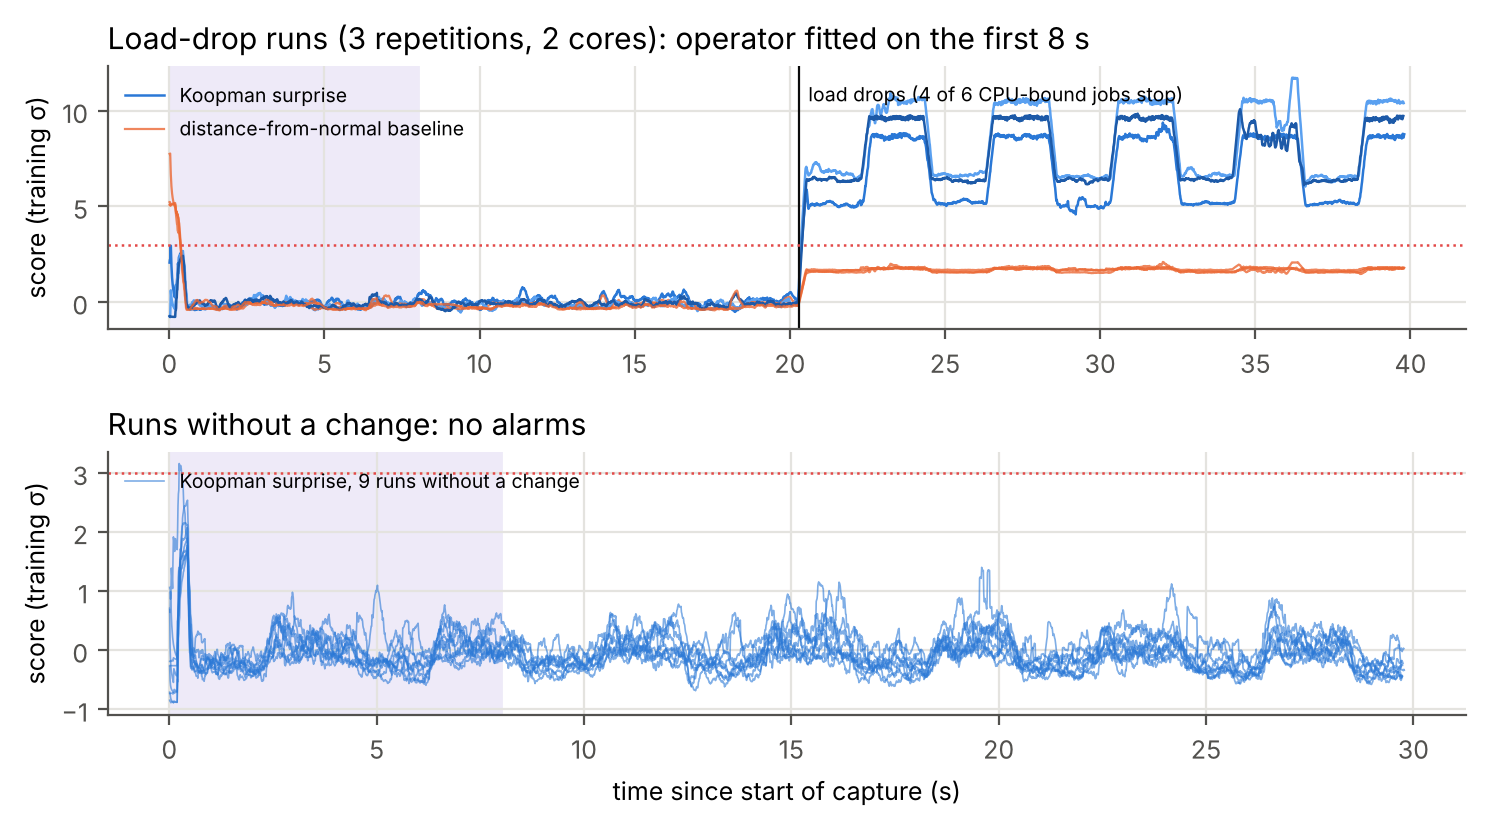
\includegraphics[width=\columnwidth]{m3_koopman_detection.png}
\caption{Trace-based detector on the VM. Top: three runs with a load drop at 20\,s. Bottom: nine runs without a change. Shaded: training.}\label{fig:regime}
\end{figure}

\section{Making the Scheduler Visible}\label{sec:viz}
The Scheduler Observatory (Fig.~\ref{fig:viz}) replays validated traces in a browser: each core is a tile lit in the colour of the task it runs, queued tasks wait under their core with growing wait bars, sleeping tasks rest in a pool, migrations are drawn as arcs, a log narrates each decision, and a Koopman panel shows the eigenvalues of a sliding-window operator and the live residual.

\begin{figure}[t]
\centering
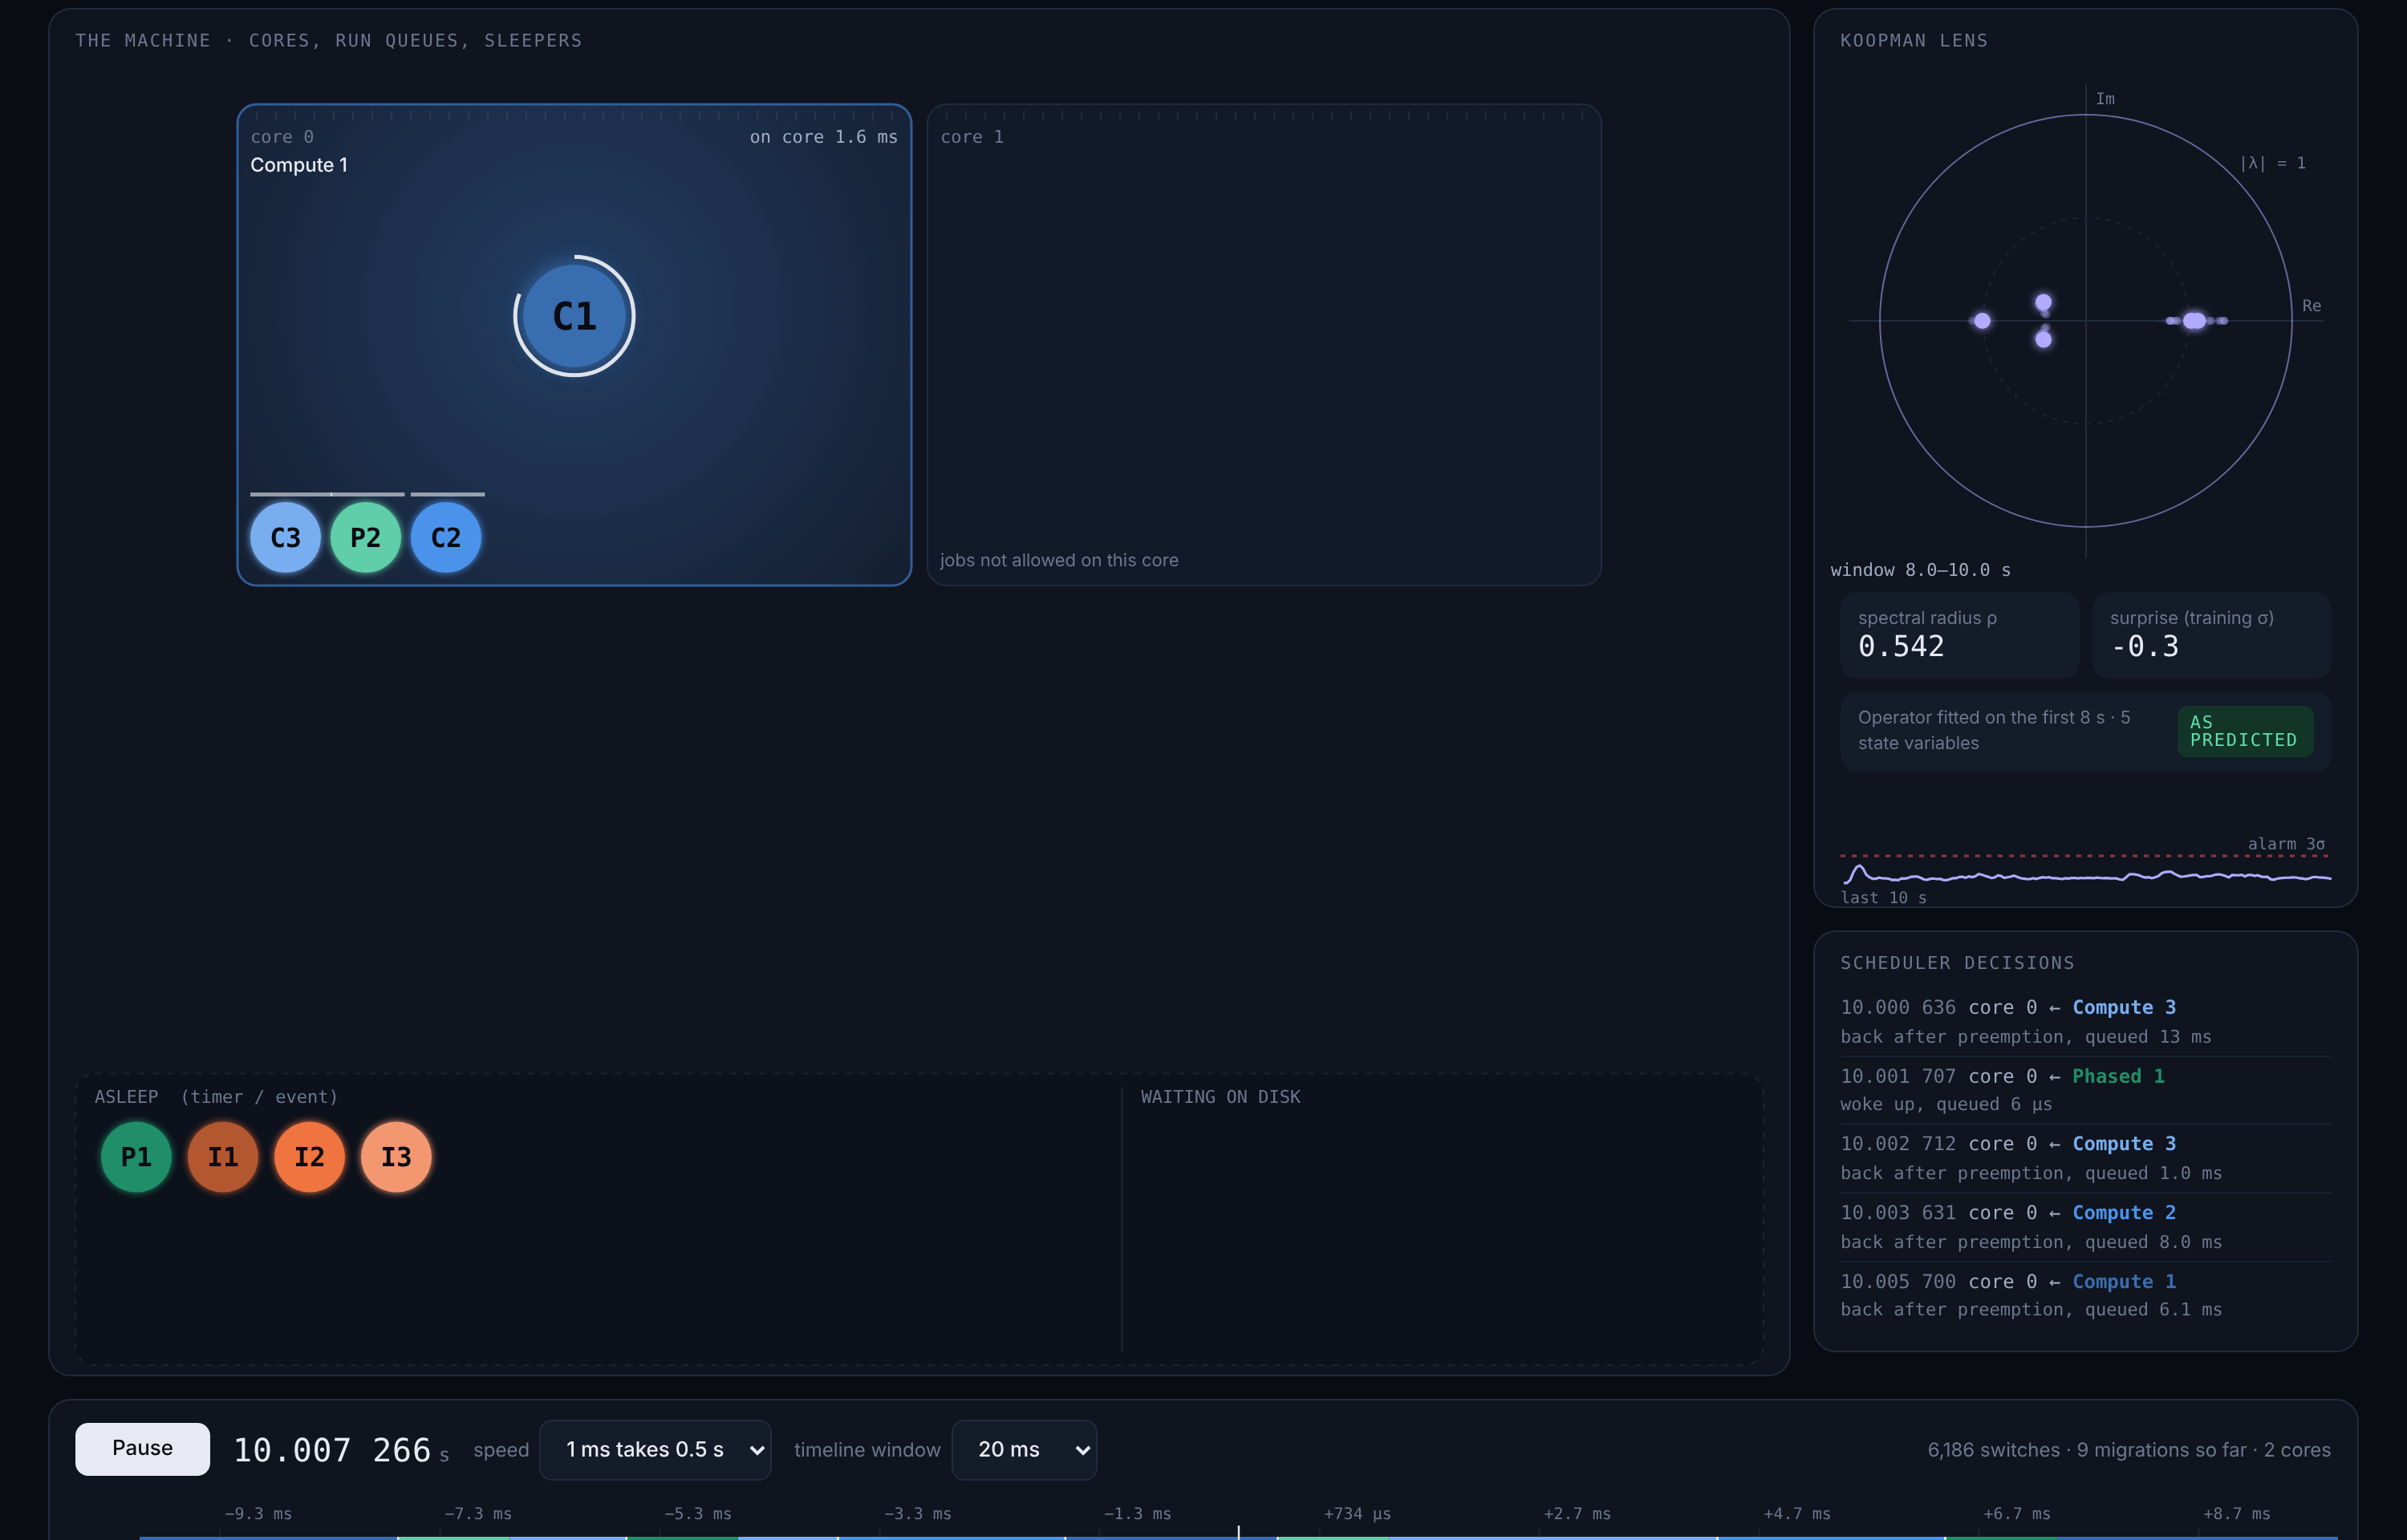
\includegraphics[width=\columnwidth]{observatory.png}
\caption{Scheduler Observatory replaying one core shared by eight jobs: running job, queued jobs with wait bars, sleepers, Koopman eigenvalues and decision log.}\label{fig:viz}
\end{figure}

\section{Beyond the Operating System}\label{sec:apps}
The same estimator has also been applied above the operating system; we summarize these as case studies. \textbf{Network traffic}~\cite{drishti2026}: 16.2 million CSE-CIC-IDS2018 flow records~\cite{sharafaldin2018} were binned into 30\,s windows with an 11-dimensional state; one $11\times11$ operator lowered forecast mean squared error against persistence on a held-out day by 25.9\% at 30\,s, 29.1\% at 60\,s and 18.9\% at 15\,min, and by 20.7\% on UNSW-NB15~\cite{moustafa2015}; its slowest mode ($\lambda=0.995$) has a half-life of 71\,min. \textbf{Markets}: EIGENWORLD~\cite{eigenworld} fits a Koopman operator on diffusion-map coordinates~\cite{coifman2006} of seven daily S\&P\,500 features. Rerun under 11 fixed seeds, 10 reproduce its published minimum of spectral entropy on 2008-08-27, 19 days before the Lehman Brothers bankruptcy, and on 1992--2026 the lowest entropy in 34 years falls in July--August 2008 for every seed (Fig.~\ref{fig:market}).

\begin{figure}[t]
\centering
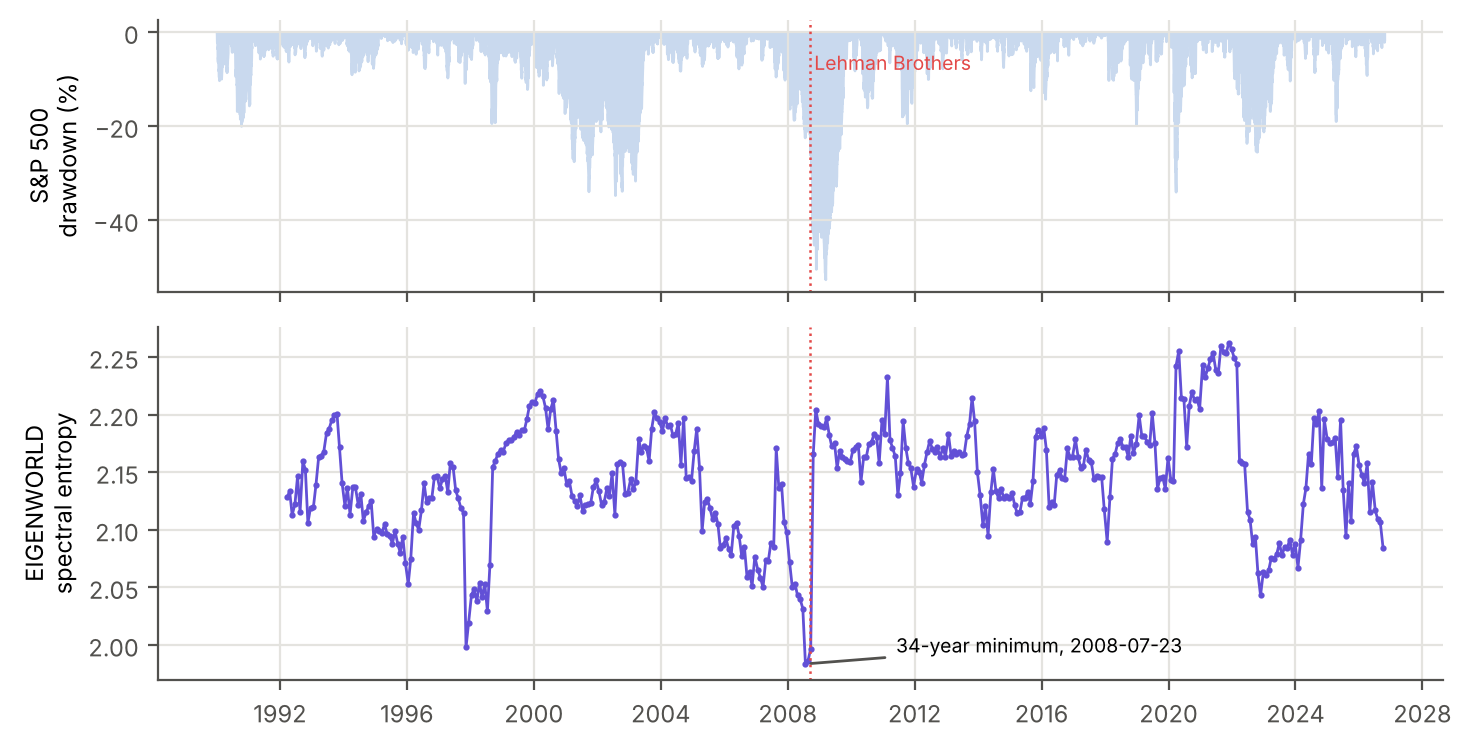
\includegraphics[width=\columnwidth]{e6_eigenworld.png}
\caption{S\&P\,500 drawdown and EIGENWORLD's spectral entropy (seed 0), 1992--2026; the 34-year minimum falls in July 2008.}\label{fig:market}
\end{figure}

\section{Discussion}
\begin{table}[t]
\centering
\caption{Summary of results}\label{tab:summary}
\setlength{\tabcolsep}{3pt}
\begin{tabular}{@{}p{2.4cm}p{3.3cm}p{2.1cm}@{}}
\toprule
Task & Result & Compared with \\
\midrule
Real-program bursts & 29\% lower error, 32/36 threads & textbook EWMA \\
Contended I/O bursts & 14\% lower error, 33/33 & textbook EWMA \\
Nonlinear observables & no gain & log-AR($p^*$) \\
Steering EEVDF (eBPF) & short requests 45\% faster, no throughput loss & stock Linux \\
Koopman vs EWMA in loop & better in 19/24 runs & EWMA predictor \\
Real servers & Redis 31--37\%, SQLite points 31\% faster; tails unchanged & stock Linux \\
Load change, traces & 3/3, 77--94\,ms & baselines 0/3 \\
Load change, live & 29/36, 0.18\,s & static score as good \\
\bottomrule
\end{tabular}
\end{table}

Table~\ref{tab:summary} collects the results. For burst prediction, the Koopman framing earns its place through the log scale, the delay coordinates and the eigenvalues, not through nonlinear observables: on scheduler data, Hankel DMD and a log-scale autoregressive model are the same predictor, and richer models add nothing. Its practical value is in the loop. Predicted bursts, turned into EEVDF slice requests with a margin of about 1.5, make short requests 40--45\% faster on a contended core, cost nothing in throughput when observed through eBPF, and speed up real servers' requests by about a third. How the forecast becomes a slice matters more than which forecaster is used: the wrong margin erases the gain even for a perfect predictor. Within that, a more accurate predictor helps where slices are tight, as the model predicts. The real-server results also show the limits: tails and heavy requests are unchanged, and for some programs a hand-set slice is better, if one knows which tasks to set.

\textbf{Threats to validity.} The closed-loop and real-program experiments ran on a 2-vCPU VM with a 250\,Hz tick and no kernel preemption; hypervisor scheduling adds noise, and the best margin may differ elsewhere. The closed-loop request workload is synthetic; the real-program loop covers three servers on one contended core. Only one bare-metal trace exists, without contention. The multi-core simulator is idealized; an EEVDF simulator we built did not reproduce the measured closed-loop effects and is not used. Network numbers come from the original study; the market result reproduces one published event.

\section{Conclusion and Future Work}
A Koopman operator on log-scale delay coordinates predicts CPU bursts better than the textbook estimator, by 29\% on real programs; it is an autoregressive model in disguise, and nonlinear observables do not improve it. Used to set EEVDF slice requests with a margin, it makes short requests up to 45\% faster on the stock Linux scheduler at negligible cost, and real server requests about a third faster. Remaining work needs bare metal: the closed loop on 8--28 cores, the real-program loop, contended scaling captures, and the frequency test that would explain the threefold I/O slowdown in Trace~3. For that test we provide a sched\_ext policy (\texttt{scx\_koopman}) that orders tasks by virtual time plus predicted burst; it compiles but has not yet been run.

\section*{Data and Code Availability}
Capture kit, eBPF observer, controller, sched\_ext policy, parsers, validation, simulators, all analyses and data (72 validated captures and counter runs, 264 closed-loop runs), the EIGENWORLD reproduction and the visualizer are at \url{https://github.com/SaarthakManocha/Koopman-Operator-Theory-Research}; its README lists the script behind each table and figure.

\balance
\bibliographystyle{IEEEtran}
\bibliography{refs}

\end{document}
